\section{Motivation}
\label{s:motivation}

% - characteristics of concurrency bugs
% - challenges / design requirements
% - limitations of existing approaches

% This work is motivated by the observation that concurrency fuzzing
% requires a new interleaving coverage metric and a better interleaving
% exploration method.
%
In this section, we first study how concurrency bugs manifest
depending on thread interleaving through a real-world concurrency bug
example.  Then, we elicit design goals to effectively discover kernel
concurrency bugs, and discuss limitations in prior work. 

%None of previous work properly addresses characteristics of \textit{offending thread interleaving} (\ie, one that causes a concurrency bug).
%
%As a consequence, previous work either \textbf{1)} disregards a
%multi-thread input in which a concurrency bug reside~\cite{krace,
  %conzzer},
%or \textbf{2)} waste the computing power by ineffectively exploring
%the search space of thread interleaving~\cite{snowboard, razzer, muzz}.

\PP{Manifestation of concurrency bugs}
%
\begin{figure}[t]
  \centering
  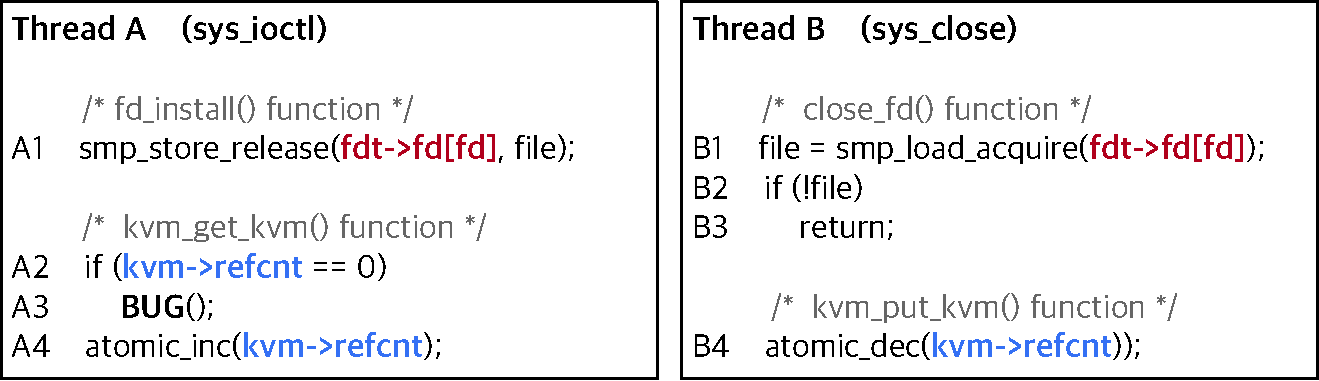
\includegraphics[width=0.85\linewidth]{fig/cve-2017-10661.pdf}
  \caption{Simplified code snippet of CVE-2017-17712. If \texttt{B1}
    is executed between \texttt{A2} and \texttt{A4}, concurrent
    accesses on \texttt{inet->hdrincl} leads to uninitialized stack
    pointer usage on \texttt{rfv}, and an attacker may gain root
    privileges through a dedicated attack
    technique~\cite{stackspray}.}
  \label{fig:cve-2017-17712}
  \vspace{-8pt}
\end{figure}
%
In \autoref{fig:cve-2017-17712}, an uninitialized access bug may
manifest when two system calls are executed concurrently:
\texttt{sendmsg()} to send a message through an ipv4 socket, and
\texttt{setsockopt()} to modify an option of the ipv4 socket.
Let us assume \texttt{inet->hdrincl} is initially \texttt{1}.
%
During sending a message through the ipv4 socket, thread~A reads a
value of \texttt{inet->hdrincl} twice at \texttt{A2} and \texttt{A4}.
%
However, since these two read operations are not atomically executed,
thread~B may intervene in the middle of these two read operations.
%
In that case, if \texttt{B1} is executed between \texttt{A2} and
\texttt{A4}, thread~A reads different values of \texttt{inet->hdrincl}
at \texttt{A2} and \texttt{A4}, and dereferences \texttt{rfv} without
initializing it at \texttt{A4}.


\PP{Observation 1: Interleaving of multiple memory accesses}
%
This example demonstrates that \textit{a specific interleaving of
  multiple instructions is necessary to cause a concurrency bug}.
  % the offending interleaving
  % causing a concurrency bug consists of multiple memory accesses}.
% combined result of multiple interleaving orders}\footnote{A
  % interleaving order denotes the execution order between a pair of
  % instructions that access the same memory object.}.
%
In the example of \autoref{fig:cve-2017-17712}, three memory accesses
are interleaved, which eventually causes the uninitialized access bug.
%
First, \texttt{A2} should be executed before \texttt{B1} (\ie,
$\texttt{A2} \Rightarrow \texttt{B1}$\footnote{In this paper,
  $\texttt{X} \Rightarrow \texttt{Y}$ denotes that \texttt{X} is
  executed before \texttt{Y}}) to make thread~A not initialize
\texttt{rfv}.
%
Second, \texttt{B1} should be executed before \texttt{A4} (\ie,
$\texttt{B1} \Rightarrow \texttt{A4}$) to make thread~A dereference
uninitialized \texttt{rfv} while other memory accesses do not
contribute to the bug.
%
%Therefore, thread interleavings satisfying a combination of the two
%interleaving orders (\ie,
%$(\texttt{A2} \Rightarrow \texttt{B1}) \wedge (\texttt{B1} \Rightarrow
%\texttt{A4}))$ cause the uninitialized access bug, while all other
%thread interleavings do not.
Therefore, to trigger the kernel concurrency bug, a fuzzer must
consider interleavings of the three memory accesses, \eg,
$(\texttt{A2} \Rightarrow \texttt{B1} \Rightarrow \texttt{A4})$.


\PP{Design goal 1: Informative interleaving coverage}
%
The observation gives an insight of how to define interleaving
coverage metric.
%
When discovering the uninitialized access bug, an interleaving
coverage metric should distinguish different interleavings of multiple
memory accesses.
%
For example,
$(\texttt{B1} \Rightarrow \texttt{A2} \Rightarrow \texttt{A4})$ (\ie,
\autoref{fig:alias-coverage}-(a)) and
$(\texttt{A2} \Rightarrow \texttt{B1} \Rightarrow \texttt{A4})$ (\ie,
\autoref{fig:alias-coverage}-(b)) should be distinguished, and thus,
interleaving coverage should not be saturated until
$(\texttt{A2} \Rightarrow \texttt{B1} \Rightarrow \texttt{A4})$ is
executed.
%
Otherwise, a fuzzer may think that there is no more interesting thread
interleaving in the multi-thread input after it executes
\autoref{fig:alias-coverage}-(a), and stop searching for new
interleavings in the input, missing the opportunity to 
find the concurrency bug.
%
However, it is crucial that how many instructions the coverage 
metric consider to distinguish different interleavings.
If interleaving coverage metric tracks interleavings 
of too few instructions (\eg, 2), it may miss interleavings 
that should be tested. On the other hand, tracking interleavings 
of too many instructions (\eg, thousands) cause high search 
complexity due to its large coveragespace.
Therefore, this work seeks a balancing point in bug-finding 
capability and search complexity 
when defining an interleaving coverage metric.

\begin{figure}[t]
  \centering
  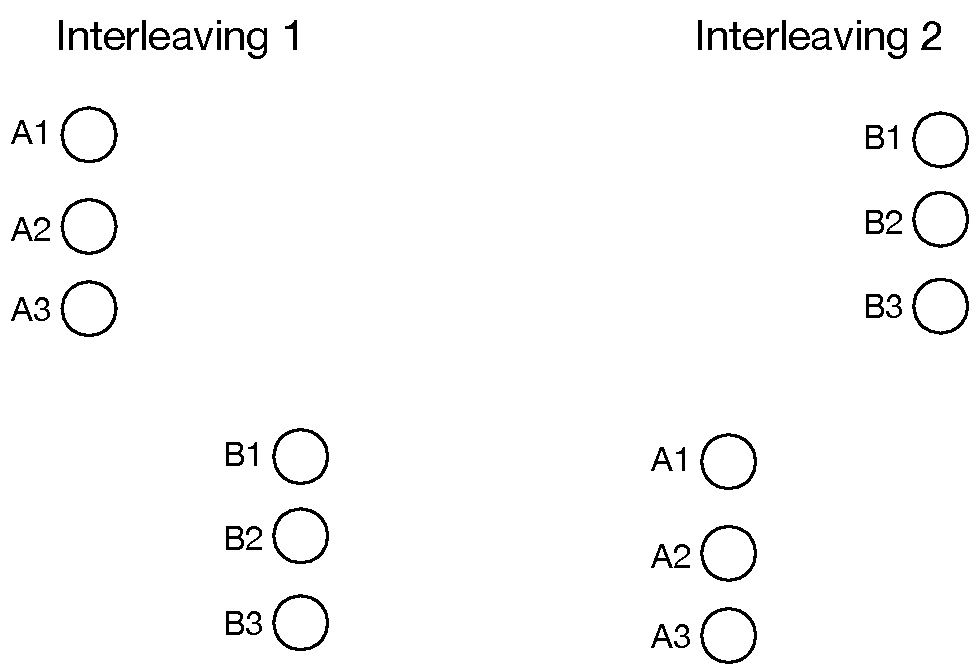
\includegraphics[width=0.8\linewidth]{fig/alias-coverage.pdf}
  \caption{Two thread interleavings between thread~A and thread~B
    described in \autoref{fig:cve-2017-17712}.
    %
    The uninitialized access bug manifests only in (b).
    %
    We omit bug-irrelevant memory accesses (\ie, \texttt{A6} and
    \texttt{B2}).}
  \label{fig:alias-coverage}
  \vspace{-8pt}
\end{figure}


\PP{Observation 2: Feedback from explored executions}
%
We find that even if an explored execution does not cause a
concurrency bug, it provides useful feedback to guide what
interleavings should be further explored.
%
In the example of \autoref{fig:cve-2017-17712}, let us assume a fuzzer
executes the two system calls \textit{sequentially} such that thread~B
executes all instructions followed by the execution of thread~A (\ie,
\autoref{fig:alias-coverage}-(a)).  In the explored execution, a
fuzzer observes the three instructions, \texttt{B1}, \texttt{A2}, and
\texttt{A4}, are executed in the order of
($\texttt{B1} \Rightarrow \texttt{A2} \Rightarrow \texttt{A4}$) and
they access the same memory object~(\ie, \texttt{inet->hdrincl}).
% \yj{can a fuzzer know they are conflicting instructions?}
%
From this execution, one can easily imagine a new interleaving of
these three instructions by changing the execution order of
\texttt{B1} and \texttt{A2}, resulting in
\autoref{fig:alias-coverage}-(b).
% $\texttt{A2} \Rightarrow \texttt{B1} \Rightarrow \texttt{A4}$).
%
The speculative interleaving is what exactly we are looking for; it is
the offending interleaving causing the uninitialized access bug, \eg,
$(\texttt{A2} \Rightarrow \texttt{B1} \Rightarrow \texttt{A4})$, and,
if executed, the interleaving triggers the bug.

\PP{Design goal 2: Speculative interleaving exploration}
%
The observation gives a direction that how a fuzzer should explore the
search space using a coverage metric.  If interleaving coverage tracks
that ($\texttt{B1} \Rightarrow \texttt{A2} \Rightarrow \texttt{A4}$)
is \textit{explored} before, a fuzzer can utilize interleaving
coverage as feedback to infer \textit{unexplored} thread interleavings
(\eg, $\texttt{A2} \Rightarrow \texttt{B1} \Rightarrow \texttt{A4}$).
%
This allows a systematic way to explore the search space rather than
performing randomized or heuristic-based exploration pervasively used
in previous approaches~\cite{ski, krace, pctalgorithm, muzz}.
% \yj{cite}
%
Considering a concurrency bugs often manifest with a thread
interleaving that rarely happen~\cite{exprace}, the systematic
interleaving exploration boosts up the concurrency bug discovery, as a
fuzzer directly executes unexplored thread interleavings instead of
executing random interleavings thousands of times.


% \dr{cut?}
%
% In summary, using the coverage metric expressing interleavings of
% multiple memory accesses and the speculative interleaving exploration,
% a fuzzer can effectively determine what to execute in future
% iterations, and quickly discover concurrency bugs without redundantly
% executing thread interleavings.


\subsection{Limitation of prior approaches}
\label{ss:existingapproaches}
%
% \begin{table}[t]
%   \centering
%   \resizebox{\linewidth}{!}{
  \begin{tabular}{l l l}
    \toprule
    & \thead{\textbf{Interleaving} \\ \textbf{coverage metric}} & \thead{\textbf{Interleaving} \\ \textbf{search strategy}} \\
    \midrule
    \textbf{Razzer~\cite{razzer}} & -- & Coverage-oblivious \\
    \textbf{Krace~\cite{krace}} & Alias coverage & Coverage-oblivious \\
    % & (single instruction pair) & \\
    \textbf{Conzzer~\cite{conzzer}} & Concurrent call pair & Coverage-based (limited) \\
    % & (single function pair) & (limited)\\
    \textbf{Snowboard~\cite{snowboard}} & -- & Coverage-oblivious \\
    \bottomrule
  \end{tabular}
}

%%% Local Variables:
%%% mode: latex
%%% TeX-master: "../p"
%%% End:

%   \caption{Interleaving coverage metrics and interleaving search
%     strategy of recent concurrency fuzzing. ``--'' indicates that a
%     fuzzer does not adopt a concurrency coverage metric. \dr{TODO:
%       rewording}}
%   \label{table:motivation}
% \end{table}

% \autoref{table:motivation} summarizes interleaving coverage metrics and 
% interleaving search strategies of prior approaches.
%
Altough prior approaches achieve their own successes, we find that
their interleaving coverage metrics and interleaving exploration
methods do not satisfy \textbf{Design goal 1} and \textbf{2}.


\PP{Less informative interleaving coverage}
%
We find that previously proposed interleaving coverage metrics are
limited in distinguishing two interleavings in
\autoref{fig:alias-coverage}.  Thus, they do not satisfy
\textbf{Design goal 1}.
%
For example, let us suppose we adopt alias coverage~\cite{krace},
which tracks interleaving orders of \textit{two} instructions.
%
Alias coverage determines an interleaved execution \texttt{X} exposes
a new behavior if \texttt{X} contains an unexplored
directed-instruction pair $I_W \rightarrow I_R$, where $I_R$ reads a
value written by $I_W$.
%
Assuming \autoref{fig:alias-coverage}-(a) is executed first, alias
coverage identifies \autoref{fig:alias-coverage}-(a) exposes new
behaviors when it sees two unexplored directed-instruction pair:
($\texttt{B1} \rightarrow \texttt{A2}$) and
($\texttt{B1} \rightarrow \texttt{A4}$).
%
% The \texttt{Interleaving \#2} is the interleaving orders causing the bug.
However, according to alias coverage,
\autoref{fig:alias-coverage}-(b), which causes the uninitialized
access bug, does not exhibit any new coverage because
($\texttt{B1} \rightarrow \texttt{A4}$) is already explored in
\autoref{fig:alias-coverage}-(a).
%
% Krace considers that growing alias coverage is a promising signal 
% to explore thread interleavings further, but the \texttt{Interleaving \#2} does not increase alias coverage in this scenario.
%But, when alias coverage faces \texttt{Interleaving \#2} after
%\texttt{Interleaving \#1}, it suffers from locating unobserved unique
%behaviors of \texttt{Interleaving \#2}, because there is no unobserved
%interleaving order in \texttt{Interleaving \#2} (\ie,
%($\texttt{B1} \Rightarrow \texttt{A4}$) is already observed in
%\texttt{Interleaving \#1}).
%
Therefore, alias coverage may make the wrong decision about whether a
fuzzer needs to run these two system calls more, misleading a fuzzer
to de-prioritize a multi-thread input in which a concurrency bug
resides. In evaluation, we quantify the limitation in
\autoref{table:aliascoverage}.
%
% \dr{I want to cut concurrenct call pair}
Likewise, concurrent call pair coverage~\cite{conzzer} also suffers
from distinguishing these two thread interleavings;
%
These two interleavings take place in the same functions (\ie,
\texttt{raw_sendmsg()} and \texttt{do_ip_setsockopt()}), while
concurrent call pair tracks a concurrently-executed function pair
without aware of fine-grained interleavings of instruction within a
function.
% %
% Since two thread interleavings in \autoref{fig:alias-coverage} take
% place in the same function (\ie, \texttt{A2} and \texttt{A4} are
% executed in the same function), concurrent call pair is also limited
% in distinguishing the two interleavings, and shows the same limitation
% as alias coverage when it comes to discovering this uninitialized
% access bug.

% is also saturated with these two thread
% interleavings, because once two functions \texttt{sendmsg()} and
% \texttt{setsockop()} are executed concurrently, concurrnet call pair
% does not matter how a thread interleaving occurs within the function
% pair.





% \yj{This paragraph must be easy enough for reader to intuitively understand, but hard to digest discussions}
% However, they are not applicable to track behavioral changes\yj{what does it mean?} according
% to a combination of interleaving orders, mainly because they either
% track only a \textit{single} interleaving order~\cite{krace, muzz} or
% \textit{coarse-grained information} such as a pair of two
% concurrently-executed functions~\cite{conzzer}.
% \yj{I do not understand why tracking a single int. order and coarse-grain information are not able to track behavioral changes}

% Taking the example of KRace's alias coverage,
% \autoref{fig:alias-coverage} describes two thread interleavings that
% saturate alias coverage found between two system calls in
% \autoref{fig:cve-2017-17712}.
% %
% In these example interleaving scenarios, the uninitialized access does
% not manifest even after alias coverage is saturated, and a fuzzer may
% decide to stop searching for new thread interleavings in the two
% system calls.
% %
% While we do not enumerate all proposed interleaving coverage metrics
% here, we find that they all share the same limitation.


\PP{Ineffective interleaving exploration}
%
Stemming from the aforementioned limitations in coverage, proposed
thread interleaving exploration methods do not efficiently explore the
search space of thread interleaving due to the lack of guidance of
their interleaving coverage (\ie, not satisfying \textbf{Design goal
  2}).
%
Specifically, Razzer~\cite{razzer} and Snowboard~\cite{snowboard} are
coverage-oblivious.  They do not make use of any interleaving
coverage, and perform their heuristic-based interleaving exploration,
which inevitably execute redundant thread interleavings.
%
KRACE~\cite{krace} randomly schedules instructions at every iteration
without considering what thread interleavings are explored before.
KRACE limitedly utilizes interleaving coverage only when deciding
whether it runs a given multi-thread input more.
% \dr{
% Whereas, we use the coverage to
% infer which thread interleavings to search further in future
% iterations.
% }
%
Whereas Conzzer~\cite{conzzer} designates two functions and run them
concurrently, but it still leaves instructions' interleaving
uncontrolled and scheduled randomly.
%
As a consequence, existing approaches do not systematically search for
thread interleavings.  Rather, they \textit{blindly} go through
trial and error, exploring thread interleavings ineffectively.

% making \textit{redundant executions} without exploring
% meaningful thread interleavings\yj{Do we measure this?}.

% %
% However, its interleaving coverage (\ie, concurrent call pair) tracks
% thread interleavings in the function-level granularity, and is limited
% in distinguishing tested interleavings and untested interleavings in
% the instruction-level granularity.
% %
% In other words, the Conzzer's interleaving search strategy can direct
% a fuzzer to execute two functions \texttt{raw_sendmsg()} and
% \texttt{do_ip_setsockopt()} concurrently.
% %
% But even after that, Conzzer suffers from triggering the uninitialized
% bug since it is not aware of the execution order of instructions.


%%% Local Variables:
%%% mode: latex
%%% TeX-master: "p"
%%% End:
